\documentclass[11pt,a4paper]{article}
\usepackage[utf8]{inputenc}
\usepackage[dvipsnames]{xcolor}
\usepackage[english]{babel}
\usepackage{listings}
\usepackage{multirow}
\usepackage{color}
\usepackage{mathrsfs}
\usepackage{hyperref}
\usepackage{biblatex} %Imports biblatex package
\addbibresource{sample.bib} %Import the bibliography file

\lstset{ %
  language=R,                     % the language of the code
  basicstyle=\footnotesize,       % the size of the fonts that are used for the code
  numbers=left,                   % where to put the line-numbers
  numberstyle=\tiny\color{gray},  % the style that is used for the line-numbers
  stepnumber=1,                   % the step between two line-numbers. If it's 1, each line
                                  % will be numbered
  numbersep=5pt,                  % how far the line-numbers are from the code
  backgroundcolor=\color{white},  % choose the background color. You must add \usepackage{color}
  showspaces=false,               % show spaces adding particular underscores
  showstringspaces=false,         % underline spaces within strings
  showtabs=false,                 % show tabs within strings adding particular underscores
  frame=single,                   % adds a frame around the codehttps://da.overleaf.com/project/5e42ac84ac4e640001f94558
  rulecolor=\color{black},        % if not set, the frame-color may be changed on line-breaks within not-black text (e.g. commens (green here))
  tabsize=2,                      % sets default tabsize to 2 spaces
  captionpos=b,                   % sets the caption-position to bottom
  breaklines=true,                % sets automatic line breaking
  breakatwhitespace=false,        % sets if automatic breaks should only happen at whitespace
  title=\lstname,                 % show the filename of files included with \lstinputlisting;
                                  % also try caption instead of title
  keywordstyle=\color{blue},      % keyword style
  commentstyle=\color{ForestGreen},   % comment style
  stringstyle=\color{mauve},      % string literal style
  escapeinside={\%*}{*)},         % if you want to add a comment within your code
  morekeywords={*,...}            % if you want to add more keywords to the set
}
\usepackage{amsmath}
\usepackage{graphicx}
\usepackage{capt-of}
\usepackage{import}
\usepackage{booktabs, array}
\usepackage{siunitx}
\usepackage{tabularx}
\usepackage{dcolumn}
\usepackage{longtable}
\usepackage{amssymb}
\usepackage{arydshln}
\usepackage{titlesec}
\graphicspath{ {pictures/} }
\addto\captionsenglish{
    \renewcommand*\contentsname{Table of Contents}
}
\usepackage{wrapfig}
\usepackage{lineno, blindtext}
\usepackage{helvet}
\usepackage{longtable}
\usepackage{fullpage}
\def\DU#1{\underline{\underline{#1}}}
\def\SU#1{\underline{#1}}
\definecolor{mygreen}{rgb}{0,0.6,0}
\usepackage{listings}

\begin{document}
\begin{titlepage} % Suppresses displaying the page number on the title page and the subsequent page counts as page 1
	\newcommand{\HRule}{\rule{\linewidth}{0.5mm}} % Defines a new command for horizontal lines, change thickness here
	
	\center % Centre everything on the page
	
	%------------------------------------------------
	%	Headings
	%------------------------------------------------
	
	\textsc{\LARGE Copenhagen Business School}\\[1.5cm] % Main heading such as the name of your university/college
	
	\textsc{\Large Statistik}\\[0.5cm] % Major heading such as course name
	
	\textsc{\large Bachelorprojekt}\\[0.5cm] % Minor heading such as course title
	
	%------------------------------------------------
	%	Title
	%------------------------------------------------
	
	\HRule\\[0.4cm]
	
	{\huge\bfseries En Generalisering af Bradley-Terry Modellen og Parameter Estimering vha. LASSO}\\[0.4cm] % Title of your document
	
	\HRule\\[1.5cm]
	
	%------------------------------------------------
	%	Author(s)
	%------------------------------------------------
	
	\begin{minipage}{0.4\textwidth}
		\begin{flushleft}
			\large
			\textit{Forfattere}\\
			Lucas Johan Boesen\\ % Your name
			Christoffer Bolvig Birch\\ % Your name
			Victor Emil Skov Lundmark\\ % Your name
		\end{flushleft}
	\end{minipage}
	~
	\begin{minipage}{0.4\textwidth}
		\begin{flushright}
			\large
			\textit{Professor}\\
			\textsc{Søren Feodor Nielsen}\\
			\textsc{}\\
			\textsc{}\\% Supervisor's name
		\end{flushright}
	\end{minipage}
	
	% If you don't want a supervisor, uncomment the two lines below and comment the code above
	%{\large\textit{Author}}\\
	%John \textsc{Smith} % Your name
	
	%------------------------------------------------
	%	Date
	%------------------------------------------------
	
	\vfill\vfill\vfill % Position the date 3/4 down the remaining page
	
	{\large{December 20, 2019}} % Date, change the \today to a set date if you want to be precise
	
	%------------------------------------------------
	%	Logo
	%------------------------------------------------
	
	%\vfill\vfill
	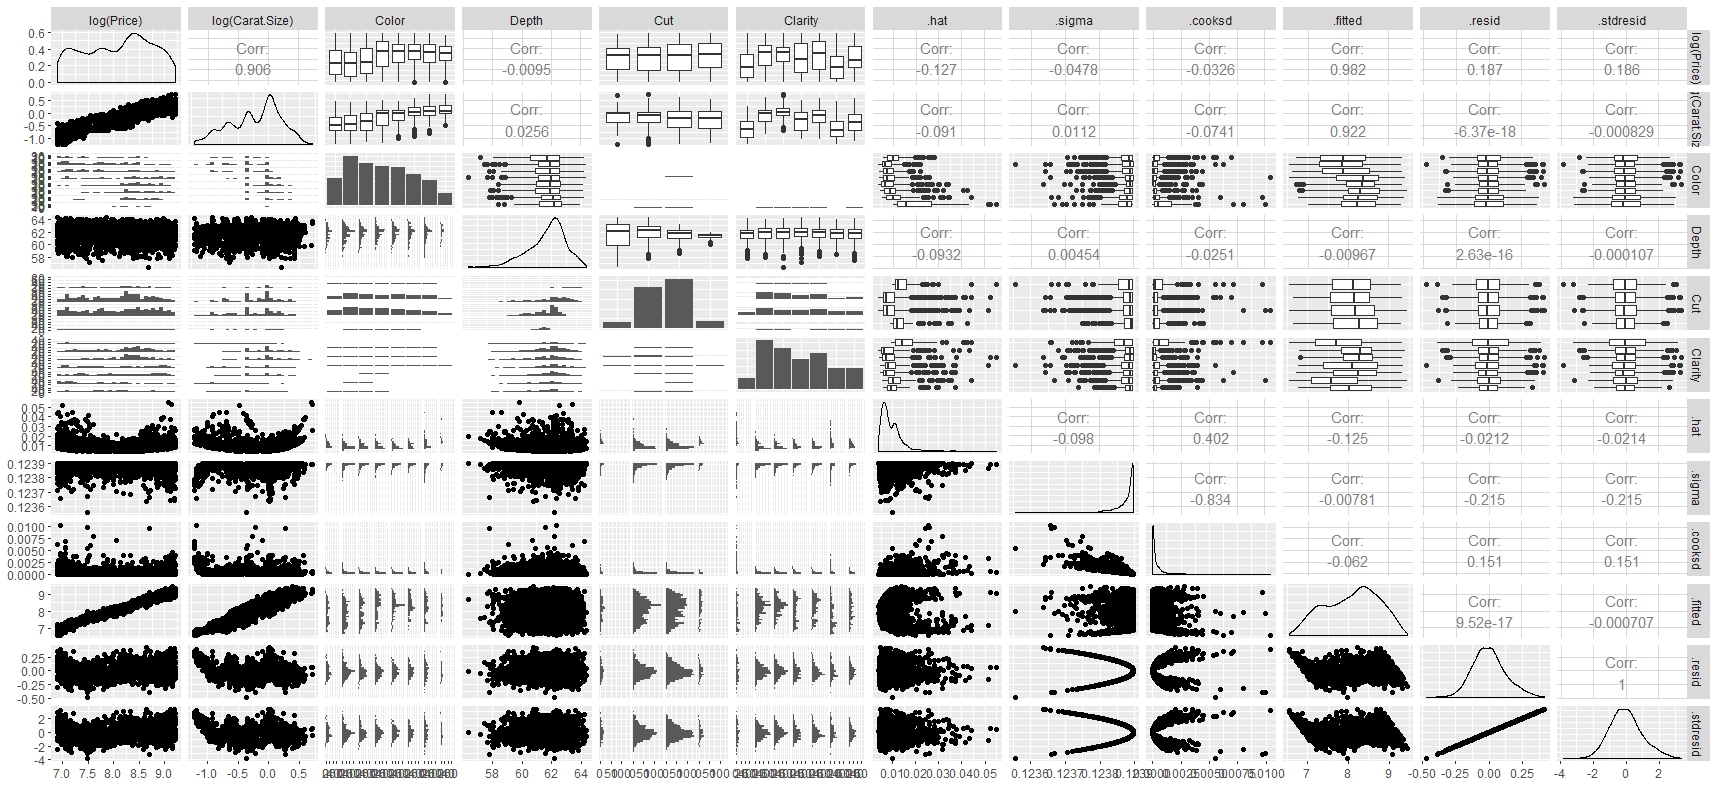
\includegraphics[width=0.8 \textwidth]{kaosmuch.png}\\[1cm] % Include a department/university logo - this will require the graphicx package
	 
	%----------------------------------------------------------------------------------------
	
	\vfill % Push the date up 1/4 of the remaining page
	
\end{titlepage}
\renewcommand{\contentsname}{Indholdsfortegnelse}
\clearpage
\tableofcontents
\clearpage
\newpage
\pagenumbering{arabic}
\begin{abstract}
Lynhurtig Bradley-Terry modellen anvendes til at lave parvise sammenligninger af f.eks. fodboldhold styrker. i den oprindelig model (Bradley \& Terry 1952) antages at der altid vil være en vinder, men da dette er en urealistisk betragtning blev modellen udvidet (Rao-Kupper 1967). til at inkludere en grænseværdiparameter som gør det muligt at indrage udfaldet uafgjort. Dette papir tager udgangspunkt i denne model og betragter anvendelsen af LASSO optimering til udvælgelsen af parametre til estimering af de forskellige holds styrke. 
\end{abstract}
\section{Generalisering af Bradley-Terry Modellen}
\subsection{Indledning}
Bradley og Terry (1952) introducerer en statistisk model til at rangere f.eks. forbrugervurderinger af produkter eller styrker af fodboldhold ved parvise sammenligninger. I først nævnte eksempel vil modellen kunne bruges til at estimere sandsynligheden for at en forbruger foretrækker et produkt over et andet og i sidst nævnte eksempel til at estimere sandsynligheden for, at Brøndby vinder over FCK i deres næste opgør. I dette papir tager vi udgangspunkt i eksemplet med sammenligninger af fodboldhold. 

\subsection{Bradley-Terry Modellen}
Når vi sammenligner hold \textit{i} med hold \textit{j} betragter vi altid situationen $i<j$, hvor vi definerer \\$i \in \{1,..,h-1\}, j\in \{i+1,...,h\}$ og \textit{h} betegner antal hold. På denne måde undgår vi at gentage parvise sammenligninger mellem hold \textit{i} og hold \textit{j}, samt at sammenligne hold med sig selv.\\
\textcolor{blue}{BT skriver} Sandsynligheden for at hold \textit{i} vinder over hold \textit{j} skrives op på formen:

\begin{center}
$P(i\ vinder\ over\ j) = p_{i\cdot ij} = \frac{\pi_i}{\pi_i+\pi_j}$,
\end{center}
hvor $p_{i\cdot ij}$ betegner sandsynligheden for at hold \textit{i} vinder over hold \textit{j}. Vi tolker $\pi_i$ og $\pi_j$ som hold \textit{i} og \textcolor{red}{-}\textit{j}'s respektive styrker. Dermed kan $Y_i=\pi_i+\epsilon_i$ betegne hold \textit{i}'s dagsform. Så hold \textit{i} vinder over hold \textit{j}, hvis $Y_i>Y_j$.\\ \textcolor{blue}{Eftersom modellens parametre kan skaleres op uden at de påvirker sandsynlighederne ses modellen at være overparameteriseret på grund af skala-invarians.} Vi kan dermed ikke identificere de enkelte styrkeparametre, men vi kan identificere forholdet mellem to styrkeparametre. For at overkomme dette problem kan der lægges et bånd på, der sikrer at vi kan estimere styrkeparametrene, dette kan gøres i form af $\pi_1 = 0$ eller $\sum_i^n \pi_i = 1$. \\
Ved omskrivning af $p_{i\cdot ij}$ kan vi udtrykke dette styrkeforhold som:
\begin{align*}
    p_{i\cdot ij} &= \frac{\pi_i}{\pi_i+\pi_j}=\frac{1}{1+\frac{\pi_j}{\pi_i}}=\frac{1}{1+e^{-(\log(\pi_i)-\log(\pi_j))}}\\
    &=F(V_{i\cdot ij})=\int_{-\infty}^{V_{i\cdot ij}} \frac{\partial p_{i\cdot ij}}{\partial V_{i\cdot ij}} \text{ d}V=\frac{1}{1+e^{-V_{i\cdot ij}}},
\end{align*}
hvor $V_{i\cdot ij}=\log(\pi_i)-\log(\pi_j)$ beskriver log-styrken for hold \textit{i} i forhold til hold \textit{j}. Det ses altså at sandsynligheden for at \textit{i} vinder over \textit{j} afhænger af forskellen i hold \textit{i} og hold \textit{j}'s styrker. Eftersom 
\begin{align*}
&f(V_{i\cdot ij})=\frac{\partial p_{i\cdot ij}}{\partial V_{i\cdot ij}} = \frac{e^{-V_{i\cdot ij}}}{(e^{-V_{i\cdot ij}}+1)^2} \geq 0, \\ \intertext{samt at}
&\int_{-\infty}^\infty f(V_{i\cdot ij}) \text{  d} V_{i\cdot ij} = 1,
\end{align*}
er $f(V_{i\cdot ij})$ en tæthed for den logistiske fordeling. Hvor $F(V_{i\cdot ij})$ er den tilhørende fordelingsfunktion, som for givne styrke parametre kan opfattes som en sandsynlighed.\\
Sandsynligheden for at hold \textit{i} vinder over hold \textit{j} på en given kampdag, tolkes som sandsynligheden for at hold \textit{i}'s dagsform er bedre (større) end hold \textit{j}'s:
\begin{align*}
p_{i\cdot ij}&=P\big{\{}y_i>y_j\big{\}}
\\&=P\big{\{}(\pi_i-\pi_j)+(\epsilon_i-\epsilon_j)>0\big{\}}
\\&=P\big{\{}(\epsilon_i-\epsilon_j)>(\pi_i-\pi_j)\big{\}}
\\&=\frac{1}{1+e^{-(log(\pi_i)-log(\pi_j))}} 
\\&=\frac{\pi_i}{\pi_i+\pi_j},\;\;
\end{align*}
\\
For at forskellene mellem fejlledene $\epsilon_i-\epsilon_j$ er logistisk fordelt skal $\epsilon_i$'erne være uafhængige og gumbel fordelte.

\subsection{Rao-Kupper Modellen}
Indtil videre har det været en antagelse at en fodboldkamp altid har haft en vinder, men dette er ikke en realistisk antagelse, da fodboldkampe kan ende uafgjort. Det samme gælder forbrugervalget mellem to produkter. Realistisk set, kan en forbruger godt være ligeglad ved valget mellem to produkter, hvis produkterne giver ham/hende tilnærmelsesvist den samme nytte. Rao og Kupper (1967) \cite{RaoKupper} foreslår en løsning på dette dilemma, ved at udvide Bradley-Terry modellen med et grænseværdiparameter $\theta$. $\theta$ betegner den forskel i dagsform der mindst skal være mellem to hold, for at der er en vinder; hvis $\|Y_i-Y_j\| < \theta$ bliver kampen uafgjort. Rao-Kupper opskrives som integralet af en tæthed ligesom Bradley-Terry, og giver sandsynlighederne:
\begin{equation}
\begin{split}
    p_{i\cdot ij}&=F(V_{i\cdot ij}-\eta)=\frac{\pi_i}{\pi_i+\theta \pi_j}\\
    p_{j\cdot ij}&=F(V_{j\cdot ij}-\eta)=1-F(V_{i\cdot ij}+\eta)=\frac{\pi_j}{\theta \pi_i+\pi_j}\\
    p_{0\cdot ij}&=F(V_{i\cdot ij}+\eta)-F(V_{i\cdot ij}-\eta)= \frac{\pi_i \pi_j(\theta^2 -1)}{(\pi_i+\theta \pi_j)(\theta \pi_i + \pi_j)} \label{Sandynligheder},
\end{split}
\end{equation}
hvor $\eta=\log(\theta)>0 \rightarrow\theta>1$ og $p_{0\cdot ij}$ er sandsynligheden for det nye udfald, uafgjort. De tre udfald er direkte sammenlignelige med et rangeringssytem, da hvert af udfaldende ikke giver samme antal point; sejr = 3 point, uafgjort = 1 point og tab = 0 point. Ligeledes kan dette overføres til rangering af produktsammenligninger; Bedre, lige og dårligere. 

\subsection{Parameter Estimering}
\textcolor{blue}{Evt. noget intro tekst}
\textcolor{blue}{Rao-Kupper er en delmodel af den almindelige multinomialfordelingsmodel.}\\
Lad \textit{h} være antal hold, og lad $X_{ij}$ være en tredimensoinel uafhængig stokastisk variabel, som repræsentere en kamp mellem hold \textit{i} og hold \textit{j}. $X_{ij}$'s, tilhørende udfaldsområde er dermed givet ved $(X_{i\cdot ij},\;X_{j\cdot ij},\;X_{0\cdot ij})$, som hhv. repræsentere sejr til hold \textit{i}, sejr til hold \textit{j} og uafgjort, hvor: 
\begin{align*}
   &P\{X_{ij}=X_{i\cdot ij}\}=p_{i\cdot ij} &&P\{X_{ij}=X_{j\cdot ij}\}=p_{j\cdot ij} &&P\{X_{ij}=X_{0\cdot ij}\}=p_{0\cdot ij}
\end{align*}
Yderligere lader vi $r_{ij}$ være antal gentagelser af $X_{ij}$ (antal kampe mellem hold \textit{i} og hold \textit{j}), samt $Y_{ij}=(Y_{i\cdot ij},Y_{j\cdot ij},Y_{0\cdot ij})$ være den tilhørende kontingenstabel givet ved:
\begin{align*}
    &Y_{i\cdot ij}=\sum_{k=1}^{r_{ij}}1_{\{X_{ijk}=X_{i\cdot ij}\}} &&Y_{j\cdot ij}=\sum_{k=1}^{r_{ij}}1_{\{X_{ijk}=X_{j\cdot ij}\}} &&Y_{0\cdot ij}=\sum_{k=1}^{r_{ij}}1_{\{X_{ijk}=X_{0\cdot ij}\}}
\end{align*}
\\
Til at estimere styrkeparametrene og $\theta$ vil vi gøre brug af maksimere likelihooden, hvor likelihood-funktionen opstilles ved multinomialfordelingen med sandsynlighederne fra (\ref{Sandynligheder}). Likelihooden for de observerede udfald bliver dermed:
\begin{align*}
\mathcal{L}(\pi_1,...,\pi_h,\theta) &= \prod_{i<j}p_{i\cdot ij}^{Y_{i\cdot ij}}p_{j\cdot ij}^{Y_{j\cdot ij}}p_{0\cdot ij}^{Y_{0\cdot ij}}\\
&= \prod_{i<j}\Big{(}\frac{\pi_i}{\pi_i+\theta\pi_j}\Big{)}^{Y_{i\cdot ij}}
\;\Big{(}\frac{\pi_j}{\pi_j+\theta\pi_i}\Big{)}^{Y_{j\cdot ij}}
\Big{(}\frac{(\theta^2-1)\pi_i \pi_j}{(\pi_i+\theta\pi_j)(\pi_j+\theta\pi_i)}\Big{)}^{Y_{0\cdot ij}}\\
&=\prod_{i<j}\Big{(}\frac{\pi_i}{\pi_i+\theta\pi_j}\Big{)}^{Y_{i\cdot ij}}
\;\Big{(}\frac{\pi_j}{\pi_j+\theta\pi_i}\Big{)}^{Y_{j\cdot ij}}
\Big{(}\frac{(\theta^2-1)\pi_i \pi_j}{(\pi_i+\theta\pi_j)(\pi_j+\theta\pi_i)}\Big{)}^{r_{ij}-{Y_{i\cdot ij}}-{Y_{j\cdot ij}}}\\
\end{align*}
\textcolor{blue}{Sidstenævnte omskrivelse er tilføjet, for at lette notationer, samt lette udledninger af afledte.}
For nemmere at kunne arbejde med likelihooden, opskriver vi log-likelihooden: 
\begin{align*}
\textit{l}(\pi,\theta)
&=\sum_{i<j}\Big{[}Y_{i\cdot ij}\log\Big{(}\frac{\pi_i}{\pi_i+\theta\pi_j}\Big{)}
+ Y_{j\cdot ij}\log\Big{(}\frac{\pi_j}{\pi_j+\theta\pi_i}\Big{)}\\
&+ (r_{ij}-Y_{i\cdot ij}-Y_{j\cdot ij}) \log\Big{(}\frac{(\theta^2-1)\pi_i \pi_j}{(\pi_i+\theta\pi_j)(\pi_j+\theta\pi_i)}\Big{)}\Big{]}
\end{align*}
Som log-likelihooden ser ud i ovenstående, er der ikke noget der hindrer negative styrker. Dog er det klart at et forhold mellem en negativ styrke og en positiv styrke vil være misvisende, hvorfor vi log-transformerer styrkerne, ved at sætte $\gamma_i=\log(\pi_i)$:\\
\begin{align*}
\textit{l}(\gamma,\theta)
&=\sum_{i<j}\Big{[}Y_{i\cdot ij}\Big{(}\gamma_i-\log(e^{\gamma_i}+\theta e^{\gamma_j})\Big{)}
+Y_{j\cdot ij}\Big{(}\gamma_j-\log(e^{\gamma_j}+\theta e^{\gamma_i})\Big{)}\\
& +(r_{ij}-Y_{i\cdot ij}-Y_{j\cdot ij}) \Big{(} \log(\theta^2-1)+\gamma_i+\gamma_j-\log(e^{\gamma_i}+\theta e^{\gamma_j})-\log(e^{\gamma_j}+\theta e^{\gamma_i})\Big{)}\\
&\text{hvor }\gamma_i=\log (\pi_i)
\end{align*}
For at bestemme maksimum-likelihood estimaterne for vores parametre, har vi valgt at gøre brug af den iterative metode, Newton-Raphson. Newton-Raphson opstilles på følgende form, med den observerede information og scorefunktionen:
\begin{align*}
v_{k+1} = v_{k} + \textit{i}(v_{k})^{-1}\textit{s}(v_{k}),
\end{align*}
hvor $v_{k}$ er en vektor bestående af vores styrkeparametre, $\pi_i$ samt $\theta$. Eftersom parvise sammenligninger i praksis, afhænger af den data der er indsamlet, vil det være nødvendigt at have et udtryk for likelihooden i form af den data der er indsamlet. For at gøre dette, definerer vi et udtryk for samtlige $\log( \pi_i)$'er (også for referencegruppen). Dette indses ved indsættelse i den lineære sammenhæng mellem styrkerne:
\begin{align*}
    p_{i\cdot ij} = \frac{1}{1+ e^{-(log(\pi_i-log(\pi_j)}} = \frac{1}{1+ e^{-\beta(x_i^T-x_j^T)}},
\end{align*}
hvor $x_i$ er den i'te søjle i designmatricen og $\beta$ er vores parameter vektor. Designmatricens \textit{i}'te søjle indeholder altså data for hold \textit{i}, hvor den \textit{k}'te række indeholder data til den \textit{k}'te parameter i parametervektoren $\beta$. \\
I vores tilfælde vil det være data der beskriver to fodboldhold, men formen vil forblive uændret hvis det er to produkter der bliver sammenlignet.
%########################################################################
%\textcolor{olive}{Vi skal her overveje, om vi hellere vil skrive pseudo algoritme, med %de afledte ift, log($\pi_i$) istedet. Vi skal efterfølgende kommentere på de betingelser %der skal være opfyldt, for at vi ved at vores algoritme rent faktisk finder MLE %estimaterne.}
%\subsection{Numerisk Estimation af parametre vha. MM-algoritme}
%Estimationen af styrkeparametrene samt $\theta$
Til at implementere dette forhold i log-likelihooden, som vi skal maksimere ud fra parametrerne, indsætter vi $\gamma_i=x_i^T\beta$:
\begin{align*}
\textit{l}(\beta,\theta)
&=\sum_{i<j}\Big{[}Y_{i\cdot ij}\Big{(}x_i^T\beta-\log(e^{x_i^T\beta}+\theta e^{x_j^T\beta})\Big{)}
+Y_{j\cdot ij}\Big{(}x_j^T\beta-\log(e^{x_j^T\beta}+\theta e^{x_i^T\beta})\Big{)}\\
& +(r_{ij}-Y_{i\cdot ij}-Y_{j\cdot ij}) \Big{(} \log(\theta^2-1)+x_i^T\beta+x_j^T\beta-\log(e^{x_i^T\beta}+\theta e^{x_j^T\beta})-\log(e^{x_j^T\beta}+\theta e^{x_i^T\beta})\Big{)}\Big{]}
\end{align*}
Første ordens betingelserne til scorefunktionen for $\beta$ og $\theta$ bliver:
\begin{align*}
\frac{\partial \ell(\beta;\theta)}{\partial \beta}&= 
\sum_{i<j}\Big{[}\Big{(}
(r_{ij}-Y_{i\cdot ij})\Big{(}-\frac{\theta e^{x_i^T\beta}}{e^{x_j^T\beta}+\theta e^{x_i^T\beta}}\Big{)}+(r_{ij}-Y_{j\cdot ij})\Big{(}\frac{\theta e^{x_j^T\beta}}{e^{x_i^T\beta}+\theta e^{x_j^T\beta}}\Big{)}\Big{)}(x_i-x_j)\Big{]},\\
\frac{\partial \ell(\beta;\theta)}{\partial \theta}&=
\sum_{i<j}
\Big{[}
 (r_{ij}-Y_{i\cdot ij}-Y_{j\cdot ij})\Big{(}\frac{2\theta}{\theta^2-1}\Big{)}\\
 &+(r_{ij}-Y_{i\cdot ij})\Big{(}-\frac{e^{x_i^T\beta}}{\theta e^{x_i^T\beta}+e^{x_j^T\beta}}\Big{)}
 +(r_{ij}-Y_{j\cdot ij})\Big{(}-\frac{e^{x_j^T\beta}}{e^{x_i^T\beta}+\theta e^{x_j^T\beta}}\Big{)}
\Big{]},\\
\end{align*}
hvor førsteordensbetingelsen ift. $\beta$ bliver en vektor med længden lig antal rækker i designmatricen. Dermed kan scorefunktionen opstilles som:
\begin{equation}
S(\beta,\theta) = \begin{bmatrix}
\frac{\partial \ell(\beta;\theta)}{\partial \beta}\\
\frac{\partial \ell(\beta;\theta)}{\partial \theta}
\end{bmatrix}
\label{score}
\end{equation}

Udledningerne til andensordsbetingelserne bliver ligeledes: 
\begin{align*}
\frac{\partial^2 \ell(\beta;\theta)}{\partial \beta^2}
&= \sum_{i<j}\Big{[}\Big{(} -\frac{(r_{ij}-Y_{i\cdot ij})}{(\theta e^{x_i^T\beta}+e^{x_j^T\beta})^2}-\frac{(r_{ij}-Y_{j\cdot ij})}{(e^{x_i^T\beta}+\theta e^{x_j^T\beta})^2}\Big{)}e^{x_i^T\beta+x_j^T\beta}\theta(x_{i}-x_{j})^2 \Big{]},\\
\frac{\partial^2 \ell(\beta;\theta)}{\partial \theta^2}
&= \sum_{i<j} 
\Big{[}
(r_{ij}-Y_{i\cdot ij}-Y_{j\cdot ij})\Big{(}-\frac{2(\theta^2+1)}{(\theta^2-1)^2}\Big{)}\\
&+(r_{ij}-Y_{i\cdot ij})\Big{(}\frac{e^{2x_i^T\beta}}{(\theta e^{x_i^T\beta}+e^{x_j^T\beta})^2}\Big{)}
+(r_{ij}-Y_{j\cdot ij})\Big{(}\frac{e^{2x_j^T\beta}}{(e^{x_i^T\beta}+\theta e^{x_j^T\beta})^2}\Big{)}\Big{]},
\\
\frac{\partial^2 \ell(\beta;\theta)}{\partial \beta\partial \theta}
&= \sum_{i<j}\Big{[}\Big{(}
-\frac{(r_{ij}-Y_{i \cdot ij})}{(\theta e^{x_i^T\beta}+e^{x_j^T\beta})^2}
+\frac{(r_{ij}-Y_{j \cdot ij})}{(e^{x_i^T\beta}+\theta e^{x_j^T\beta})^2}\Big{)}e^{x_i\beta+x_j\beta}(x_{i}-x_{j})\Big{]},
\end{align*}
hvorved vi nu får at andenordensbetingelsen ift.$\beta$ bliver en kvadratisk matrice, hvorfor den observerede informationen opskrives som en symmetrisk blok-matrix på formen
\begin{equation}
i(\beta,\theta) = -\begin{bmatrix}
\frac{\partial^2 \ell(\beta;\theta)}{\partial \beta^2} &\frac{\partial^2 \ell(\beta;\theta)}{\partial \beta \partial \theta} \\
\Big{(}\frac{\partial^2 \ell(\beta;\theta)}{\partial \beta \partial \theta}\Big{)}^T & \frac{\partial \ell(\beta;\theta)}{\partial \theta^2}
\end{bmatrix}
\label{inf}
\end{equation}
Likelihooden konvergerer mod et maksimum givet scorefunktionen (\ref{score}) og den observerede information (\ref{inf}), hvis den observerede info(\ref{inf}) er positiv semi-definit. Da $i(\beta,\theta)$ er symmetrisk kan vi benytte Albert (1969;1972)'s Theorem \\\textbf{ THEOREM 9.1.6:} \textit{Lad A være symmetrisk, så:}
\begin{flalign*}
&M = \begin{bmatrix}
A & B\\
C & D
\end{bmatrix}\geq 0 \iff &\\
&(i)\; D\geq0\\
&(ii)\; C=D^{-1}DC\\
&(iii)\; A\geq BD^{-1}C\\
\end{flalign*}  
ad (\textit{i}): 
Vi ønsker at vise; $-\frac{\partial^2 \ell(\beta;\theta)}{\partial \theta^2} \succ 0 \text{ og } \iff (r_{ij}- Y_{i\cdot ij}-Y_{j\cdot ij}) \frac{2(\theta^2+1)}{(\theta^2-1)^2}>(r_{ij}-Y_{i\cdot ij})p_{i\cdot ij}^2 + (r_{ij}-Y_{j\cdot ij})p_{j\cdot ij}^2$. Det antages, at vi har mindst én uafgjort kamp i det datasæt vi undersøger, $(r_{ij}- Y_{i\cdot ij}-Y_{j\cdot ij}) > 0$.
\\Observation I: Når $Y_{0\cdot ij}$ bliver meget lille konvergerer $\theta$ mod 1, det medfører venstre siden i uligheden bliver numerisk stor. $p_{i\cdot ij}^2$ og $p_{j\cdot ij}^2$ vil også blive større, men de to kvadrerede sandsynligheder vil stadig have en sum mindre end 1.\\
Observation II: Når $Y_{0\cdot ij}$ er meget stor vil både venstre og højre side konvergere mod 0. Dette ses for venstresiden da $\theta$ går mod  $\infty$, og for højresiden da sandsynlighederne for sejr til hold $i$ og $j$ går mod 0. Hvilken af dem der vægter højest kan ikke siges uden konkrete observationer for $Y$'erne. Dog vil tilfældet hvor $Y_{0 \cdot ij}$ er større end $Y_{i \cdot ij} \text{ og } Y_{j \cdot ij}$ for mange hold, være yderst sjældent da udfaldet uafgjort ikke fremkommer så hyppigt, som de andre to tilsammen.\\
ad (\textit{ii}): Det er klart at, da $D$ er endimensionel er D altid invertibel, og dermed $D D^{-1}=1 \rightarrow C=C$.\\
ad (\textit{iii}):
Det er klart at A i vores tilfælde altid vil være positiv, da $-\frac{\partial^2 \ell(\beta;\theta)}{\partial \beta^2}$ kun består af positive led.
Derudover har vi at $BD^{-1}C$ også er positiv, da $D^{-1}>0$ eftersom D i vores tilfælde er endimensionelt, samt at eftersom B og C altid vil have samme fortegn, vil deres produkt være positivt. Hvorvidt denne ulighed er opfyldt, vil 
i høj grad komme an på fordelingen af $Y$'erne. \\\\
Det kan altså ikke konkluderes at vores observerede information er positiv semi-definit for samtlige $\theta$'er. Hvorimod $\beta$'erne for et låst $\theta$, vil konvergere, (da A altid er positiv). \\
For at være sikker på, at vores log-likelihood konvergerer mod et maksimum, kan der gøres en af følgende tiltag:\\
1) Finde Profillikelihooden for $\beta$'erne, hvor $\theta$ holdes fast.\\
2) For hvert skridt i Newton-Raphton tjekkes der for om det givne $\theta$, opfylder \textit{i), iii)} fra theoremet 9.1.6.\\
I praksis vil tiltag 2), være mere medgørelig at implementere, eftersom 1) vil kræve markant flere iterationer, da der først skal itereres over $\beta$'erne og derefter over $\theta$. Eftersom vi ikke ved præcist hvordan $\theta$ vil opføre sig, vil det være en god idé at implementere en skridthalvering. Hvis $\theta$ bevæger sig ud af mængden der ikke opfylder betingelserne, kan man iterere tilbage, hvor hvert skridt halveres yderligere, indtil vi er inde i mængden igen. Metoden til at finde profillikelihooden i praksis ville være at udføre Newton-Raphson hvor $\theta$ er i et interval, eksempelvis fra 1.01 til 2. Hvis der ikke findes et maksimum, kan man udvide dette interval.

\subsection{Hypotesetest af modellen}
Eftersom modellen skal anvendes i praksis, vil det være nødvendigt at teste den, for at verificere at den teoretiske model kan anvendes med en vis sikkerhed på det givne data. Det er antaget at det valgte datasæt er komplet, repræsentativt og stort. \\
På trods af at dataet er valgt ud fra forventningen, om at de beskrivende variable afspejler forholdet mellem holdenes styrker, kan dette ikke antages at være gældende. For at verificere at dataet er beskrivende, vil vi gøre brug af en log-likelihood ratio test på parametrene, på formen:\\
$H_0: \hat{\beta} = 0$\\
Hvis der ikke er evidens for at $\hat{\beta}$'erne er forskellige fra 0, vil det betyde at holdenes styrker ikke har nogen indflydelse på udfaldene (da alle styrkerne vil blive ens). Vi sætter dermed vores test-statistik op, hvor log-likelihooden maksimeres ift. $\theta$ med $\hat{\beta}$ holdt fast lig 0:\\
\begin{align*}
LR = -2\Big{(}\ell (\beta_{MLE},\theta_{MLE})-\text{max}_\theta \;\ell (\beta_{H_0},\theta)\Big{)}
\end{align*}
Her antages det at for store stikprøver er LR omtrent $\chi^2$-fordelt, med $(k-1)$ frihedsgrader. \\
Vi undlader at teste for om $\theta=1$, da den udvidede model dermed bliver nyttesløs, eftersom udfaldet uafgjort vil være udeladt fra modellen. \\\\
HER
\textbf{standardfejl for de forklarende variable ($\beta$'er) og grænseværdiparameter $\theta$}
Først opstilles dispersionsmatricen $\hat{\Sigma}$(kovariansmatricen): \textcolor{blue}{**Mener at fordi det er numerisk kan vi godt bruge observationen, ellers skal vi lige have beregnet fisher informationen og brugt den i stedet*** }
\begin{align*}
&\hat{\Sigma}=i(\beta,\theta)^{-1}=
\Big{(}-\begin{bmatrix}
\frac{\partial^2 \ell(\beta;\theta)}{\partial \beta^2} &\frac{\partial^2 \ell(\beta;\theta)}{\partial \beta \partial \theta} \\
\Big{(}\frac{\partial^2 \ell(\beta;\theta)}{\partial \beta \partial \theta}\Big{)}^T & \frac{\partial \ell(\beta;\theta)}{\partial \theta^2}
\end{bmatrix}\Big{)}^{-1}\\
\end{align*}
\begin{align}
\intertext{Standardfejlene $\hat{\sigma}_\beta$ og $\hat{\sigma}_\theta$ findes ved kvadratroden af diagonalen af $\hat{\Sigma}$}
\hat{\sigma}_{\beta,\theta}=\sqrt{\text{diag}(\hat{\Sigma})}=
\begin{bmatrix}
\hat{\sigma}_{\beta_1}& &\\
& \ddots & \\
& & \hat{\sigma}_{\beta_k} \\
& & & \hat{\sigma}_{\theta}
\end{bmatrix}
\end{align}
Modellen kan i sin helhed testes ved en $\chi^2$ Goodness of Fit test, hvor vi kan teste de kumulerede sandsynligheder op imod de observerede sandsynligheder fra kontingenstabellen. Vi kan opstille en kontingenstabel for de forventede udfald ud $\hat{Y}_{ij} = (\hat{Y}_{i\cdot ij},\hat{Y}_{j\cdot ij},\hat{Y}_{0\cdot ij})$, som er udregnet ved brug af de estimerede $\hat{\beta}$ og $\hat{\theta}$:
%For at tjekke modellen igennem er det praktisk udregne residualerne:
\begin{align*}
&\textbf{Rå (respons) residualer}\\
&\epsilon_{i\cdot ij}=Y_{i\cdot ij}-r_{ij}p_{i\cdot ij}
&&\epsilon_{j\cdot ij}=Y_{i\cdot ij}-r_{ij} p_{j\cdot ij}
&&\epsilon_{0\cdot ij}=Y_{0\cdot ij}-r_{ij} p_{0\cdot ij}\\
&\epsilon_{i\cdot ij}=Y_{i\cdot ij}-r_{ij} \frac{\pi_i}{\pi_i+\theta \pi_j}
&&\epsilon_{j\cdot ij}=Y_{i\cdot ij}-r_{ij} \frac{\pi_j}{\theta \pi_i+ \pi_j}
&&\epsilon_{0\cdot ij}=Y_{0\cdot ij}-r_{ij} \frac{(\theta^2-1)\pi_i\pi_j}{(\pi_i+\theta \pi_j)(\theta
\pi_i + \pi_j)}\\
\end{align*}
\begin{align*}
&\hat{Y}_{i\cdot ij} = r_{ij}\frac{e^{x_i^T\beta}}{e^{x_i^T\beta}+\theta e^{x_j^T\beta}},
&&\hat{Y}_{j\cdot ij} = r_{ij}\frac{e^{x_j^T\beta}}{e^{x_j^T\beta}+\theta e^{x_i^T\beta}},
&&\hat{Y}_{0\cdot ij} = r_{ij}\frac{(\theta^2-1)e^{x_i^T\beta}e^{x_j^T\beta}}{(e^{x_i^T\beta}+\theta e^{x_j^T\beta})(e^{x_i^T\beta}\theta +e^{x_j^T\beta})}.
\end{align*}
Vores $\chi^2$ teststørrelse bliver:
\begin{align*}
\chi^2 = \sum_{i<j} \frac{(Y_{i\cdot ij}-\hat{Y}_{i\cdot ij})^2}{\hat{Y}_{i\cdot ij}} + \frac{(Y_{j\cdot ij}-\hat{Y}_{j\cdot ij})^2}{\hat{Y}_{j\cdot ij}} + \frac{(Y_{0\cdot ij}-\hat{Y}_{0\cdot ij})^2}{\hat{Y}_{0\cdot ij}}
\end{align*}
Her vil det også gælde for tilstrækkeligt store stikprøver at teststørrelsen er $\chi^2$ fordelt, og her med $(h^2-2h)$ frihedsgrader. \\
Ovenstående tests skal evalueres med en vis forsigtighed, eftersom antagelsen om at den underliggende fordeling er logistisk, ikke altid vil være opfyldt. Derfor er det vigtigt at kigge på dem som en helhed, og ydermere ved brug af et PP-plot, hvor vi kigger på den teoretiske fordeling op imod vores estimerede udfald. 

\section{Tests af den udvidede Bradley-Terry model}
I denne del, vil vi teste modellen på historisk data fra den danske 3F Superliga. Der er i alt 14 hold i ligaen for hver sæson, hvor der i slutningen af sæsonen rykker ét hold op fra 1. Divison og ét hold rykker ned. Derfor vil data for to sæsoner give 16 forskellige hold.  
Tests:
Log-likelihood ratio
Plot af kumulerende observationer op mod kumulerende sandsynligheder
Derefter
Konfidensinterval på parametrene
\clearpage
\section{LASSO Regression}

\printbibliography %Printer referencer

\end{document}